\documentclass[a4paper,14pt, unknownkeysallowed]{extreport}

\usepackage{cmap} % Улучшенный поиск русских слов в полученном pdf-файле
\usepackage[T2A]{fontenc} % Поддержка русских букв
\usepackage[utf8]{inputenc} % Кодировка utf8
\usepackage[english,russian]{babel} % Языки: русский, английский
\usepackage{enumitem}


\usepackage{threeparttable}

\usepackage[14pt]{extsizes}

\usepackage{caption}
\captionsetup{labelsep=endash}
\captionsetup[figure]{name={Рисунок}}

% \usepackage{ctable}
% \captionsetup[table]{justification=raggedleft,singlelinecheck=off}

\usepackage{amsmath}

\usepackage{geometry}
\geometry{left=20mm}
\geometry{right=10mm}
\geometry{top=20mm}
\geometry{bottom=20mm}

\usepackage{titlesec}
\titleformat{\section}
	{\normalsize\bfseries}
	{\thesection}
	{1em}{}
\titlespacing*{\chapter}{0pt}{-30pt}{8pt}
\titlespacing*{\section}{\parindent}{*4}{*4}
\titlespacing*{\subsection}{\parindent}{*4}{*4}

\usepackage{setspace}
\onehalfspacing % Полуторный интервал

\frenchspacing
\usepackage{indentfirst} % Красная строка

\usepackage{titlesec}
\titleformat{\chapter}{\LARGE\bfseries}{\thechapter}{20pt}{\LARGE\bfseries}
\titleformat{\section}{\Large\bfseries}{\thesection}{20pt}{\Large\bfseries}

\usepackage{multirow}
\usepackage{listings}
\usepackage{xcolor}

% Для листинга кода:
\lstset{ %
language=caml,                 % выбор языка для подсветки (здесь это С)
basicstyle=\small\sffamily, % размер и начертание шрифта для подсветки кода
numbers=left,               % где поставить нумерацию строк (слева\справа)
stepnumber=1,                   % размер шага между двумя номерами строк
numbersep=5pt,                % как далеко отстоят номера строк от подсвечиваемого кода
showspaces=false,            % показывать или нет пробелы специальными отступами
showstringspaces=false,      % показывать или нет пробелы в строках
showtabs=false,             % показывать или нет табуляцию в строках
frame=single,              % рисовать рамку вокруг кода
tabsize=2,                 % размер табуляции по умолчанию равен 2 пробелам
captionpos=t,              % позиция заголовка вверху [t] или внизу [b] 
breaklines=true,           % автоматически переносить строки (да\нет)
breakatwhitespace=false, % переносить строки только если есть пробел
escapeinside={\#*}{*)}   % если нужно добавить комментарии в коде
}



% plot
\usepackage{graphicx}
\usepackage{pgfplots}
\usepackage{filecontents}
\usetikzlibrary{datavisualization}
\usetikzlibrary{datavisualization.formats.functions}

\graphicspath{ {img/} }


\usepackage{subcaption}

\captionsetup{labelsep=endash}
\captionsetup[figure]{name={Рисунок}}



\usepackage[justification=centering]{caption} % Настройка подписей float объектов

\usepackage[unicode,pdftex]{hyperref} % Ссылки в pdf
\hypersetup{hidelinks}

\usepackage{csvsimple}

\newcommand{\code}[1]{\texttt{#1}}

\begin{document}
	
\begin{titlepage}
	\newgeometry{pdftex, left=2cm, right=2cm, top=2.5cm, bottom=2.5cm}
	\fontsize{12pt}{12pt}\selectfont
	\noindent \begin{minipage}{0.15\textwidth}
		
\includegraphics[width=\linewidth]{img/main_logo.jpg}
	\end{minipage}
	\noindent\begin{minipage}{0.9\textwidth}\centering
		\textbf{Министерство науки и высшего образования Российской Федерации}\\
		\textbf{Федеральное государственное бюджетное образовательное учреждение высшего образования}\\
		\textbf{«Московский государственный технический университет имени \newline Н. Э. Баумана}\\
		\textbf{(национальный исследовательский университет)»}\\
		\textbf{(МГТУ им. Н. Э.~Баумана)}
	\end{minipage}
	
	\noindent\rule{18cm}{3pt}
	\newline\newline
	\noindent ФАКУЛЬТЕТ $\underline{\text{«Информатика и системы управления»~~~~~~~~~~~~~~~~~~~~~~~~~~~~~~~~~~~~~~~~~~~~~~~~~~~~~~~}}$ \newline\newline
	\noindent КАФЕДРА $\underline{\text{«Программное обеспечение ЭВМ и информационные технологии»~~~~~~~~~~~~~~~~~~~~~~~}}$\newline\newline\newline\newline\newline\newline\newline
	
	
	\begin{center}
		\noindent\begin{minipage}{1.3\textwidth}\centering
		\Large\textbf{   ~~~ Лабораторная работа №2}\newline
		\textbf{по дисциплине "Анализ Алгоритмов"}\newline\newline\newline
		\end{minipage}
	\end{center}
	
	\noindent\textbf{Тема} 			$\underline{\text{Умножение матриц}}$\newline\newline
	\noindent\textbf{Студент} 		$\underline{\text{Светличная А.А.}}$\newline\newline
	\noindent\textbf{Группа} 		$\underline{\text{ИУ7-53Б}}$\newline\newline
	\noindent\textbf{Преподаватель} $\underline{\text{Волкова Л. Л., Строганов Ю.В.}}$\newline
	
	\begin{center}
		\vfill
		Москва~---~\the\year
		~г.
	\end{center}
	\restoregeometry
\end{titlepage}
	
	\setcounter{page}{2}
	\tableofcontents
	
	\newpage
	\chapter*{Введение}
	
\addcontentsline{toc}{chapter}{Введение}
Сегодня термин «матрица» применяется во множестве разных областей: от
программирования до кинематографии. Матрица в математике – это таблица чисел, состоящая из определенного количества строк и столбцов. 
Операции обработки матриц, а в частности их умножение, является одной из самых фундаментальных операций в современных вычислениях. Умножение двух матриц возможно, если число столбцов первой матрицы совпадает с числом строк во второй. Результирующая матрица будет иметь столько же строк, сколько в первой матрице, и столько же столбцов, сколько во второй.
	
\chapter{Аналитическая часть}
	
\section{Цель и задачи}
	
Целью данной работой является изучение и реализация алгоритмов умножения матриц (стандартный алгоритм умножения матриц, алгоритм Винограда и оптимизированный алгоритм Винограда), вычисление их трудоемкости. Для достижения поставленной цели требуется решить следующие задачи:
	
\begin{enumerate}
	\item[1)] изучить и рассмотреть стандартный алгоритм умножения матриц, алгоритм Винограда и оптимизированный алгоритм Винограда; 
	\item[2)] построить блок-схемы данных алгоритмов;
	\item[3)] реализовать каждый из алгоритмов;
	\item[4)] оценить трудоемкость алгоритмов;
	\item[5)] экспериментально оценить временные характеристики алгоритмов;
	\item[6)] сделать вывод на основании проделанной работы.
\end{enumerate}

\section{Стандартный алгоритм умножения матриц}

Пусть даны две прямоугольные матрицы:
\begin{equation}
	A_{mk} = \begin{pmatrix}
		a_{11} & a_{12} & \ldots & a_{1k}\\
		a_{21} & a_{22} & \ldots & a_{2k}\\
		\vdots & \vdots & \ddots & \vdots\\
		a_{m1} & a_{m2} & \ldots & a_{mk}
	\end{pmatrix},
	\quad
	B_{kn} = \begin{pmatrix}
		b_{11} & b_{12} & \ldots & b_{1n}\\
		b_{21} & b_{22} & \ldots & b_{2n}\\
		\vdots & \vdots & \ddots & \vdots\\
		b_{k1} & b_{k2} & \ldots & b_{kn}
	\end{pmatrix}.
\end{equation}

\clearpage

Тогда матрица $C$:
\begin{equation}
	C_{mn} = \begin{pmatrix}
		c_{11} & c_{12} & \ldots & c_{1n}\\
		c_{21} & c_{22} & \ldots & c_{2n}\\
		\vdots & \vdots & \ddots & \vdots\\
		c_{m1} & c_{m2} & \ldots & c_{mn}
	\end{pmatrix},
\end{equation}

где
\begin{equation}
	\label{eq:M}
	c_{ij} =
	\sum_{r=1}^{k} a_{ir}b_{rj} \quad (i=\overline{1,m}; j=\overline{1,n}),
\end{equation}

будет называться произведением матриц $A$ и $B$. Стандартный алгоритм реализует данную формулу.


\section{Алгоритм Копперсмита-Винограда}

Алгоритм Копперсмита-Винограда — алгоритм умножения квадратных матриц, предложенный в 1987 году Д. Копперсмитом и Ш. Виноградом.
В исходной версии асимптотическая сложность алгоритма составляла $O(n^{2,3755})$, где  $n$ — размер стороны матрицы.
Алгоритм Копперсмита — Винограда, с учетом серии улучшений и доработок в последующие годы, обладает лучшей асимптотикой среди известных алгоритмов умножения матриц.

Рассмотрим два вектора $V = (v_1, v_2, v_3, v_4)$ и $W = (w_1, w_2, w_3, w_4)$.
Их скалярное произведение равно: $V \cdot W = v_1w_1 + v_2w_2 + v_3w_3 + v_4w_4$, что эквивалентно (\ref{for:new}).
\begin{equation}
	\label{for:new}
	V \cdot W = (v_1 + w_2)(v_2 + w_1) + (v_3 + w_4)(v_4 + w_3) - v_1v_2 - v_3v_4 - w_1w_2 - w_3w_4.
\end{equation}

Несмотря на то, что второе выражение требует вычисления большего количества операций, чем первое: вместо четырех умножений - шесть, а вместо трех сложений - десять, выражение в правой части последнего равенства допускает предварительную обработку: его части можно вычислить заранее и запомнить для каждой строки первой матрицы и для каждого столбца второй, что позволяет выполнять для каждого элемента лишь первые два умножения и последующие пять сложений, а также дополнительно два сложения.

Из-за того, что операция сложения быстрее операции умножения в ЭВМ, на практике алгоритм работает быстрее стандартного.

\section{Оптимизированный алгоритм Копперсмита-Винограда}

Оптимизации алгоритма:
\begin{enumerate}
	\item[1)] операции вида $x = x + k$ заменены на $x += k$;
	\item[2)] умножение 2 заменено побитовым сдвигом;
	\item[3)] происходит предвычисление некоторых слагаемых алгоритма.
\end{enumerate}
	
	
\section*{Вывод}
	
Были рассмотрены стандартный алгоритм умножения матриц, алгоритм Винограда и оптимизированный алгоритм Винограда. Основное отличие алгоритмов Винограда от стандартного алгоритма — наличие предварительной обработки, а также количество операций умножения.
	
\clearpage
	
\chapter{Конструкторская часть}

\section{Описания алгоритмов}
	
На рисунках ниже показаны схемы стандартного алгоритма умножения матриц, алгоритма Винограда и оптимизированного алгоритма Винограда.

\begin{figure}[h!]
	\centering
	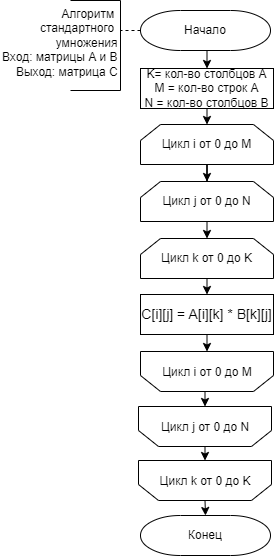
\includegraphics[scale=0.95]{img/std_mul.png}
	\caption{Схема стандартного алгоритма умножения матриц}
	\label{fig:std_mul}
\end{figure}

\clearpage

\begin{figure}[h!]
	\centering
	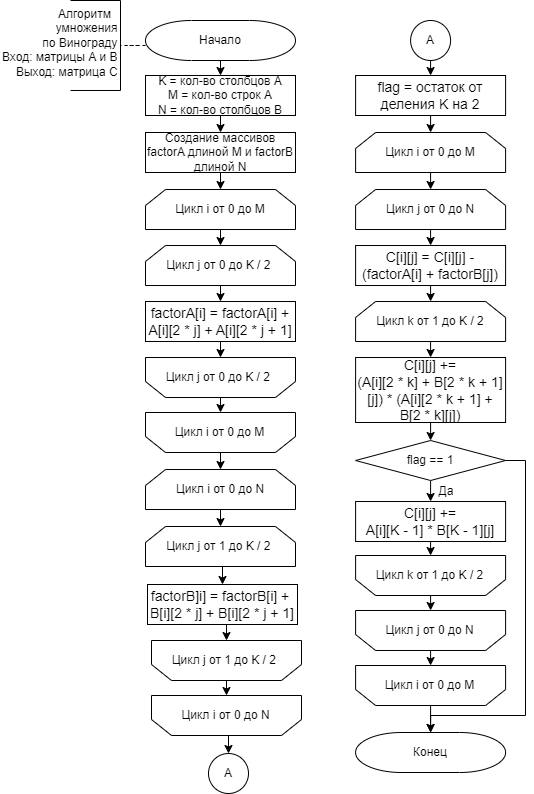
\includegraphics[scale=0.9]{img/wino.png}
	\caption{Схема алгоритма Винограда}
	\label{fig:wino}
\end{figure}

\clearpage

\begin{figure}[h!]
	\centering
	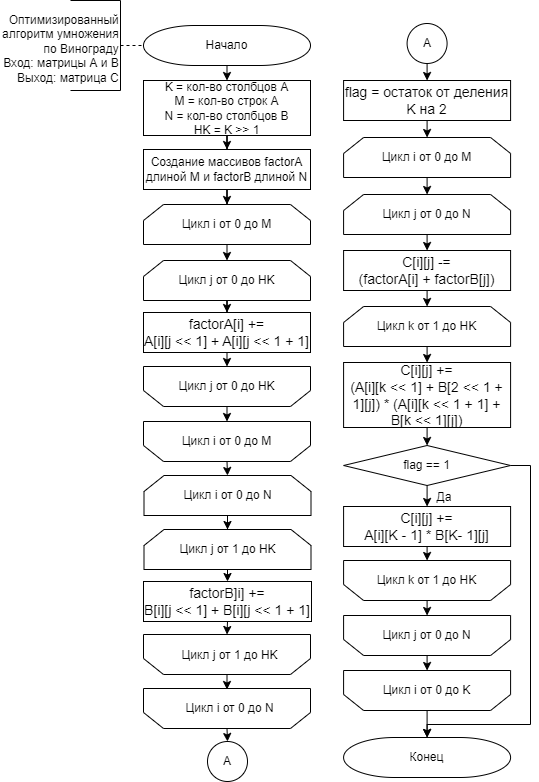
\includegraphics[scale=0.9]{img/opt_wino.png}
	\caption{Схема оптимизированного алгоритма Винограда}
	\label{fig:wino}
\end{figure}

\clearpage
	
\section{Модель вычислений трудоемкости}

\begin{enumerate}
	\item[1)] Операции, имеющие трудоемкость 1:
	\begin{equation*}
	   +, -, \%, ==, !=, <, >, <=, >=, [], ++, {-}-, {<}<, {>}>.
	\end{equation*}
	\item[2)] Операции, имеющие трудоемкость 2:
	\begin{equation*}
		*, /.
	\end{equation*}
	\item[3)] Трудоемкость оператора выбора if условие then A else B рассчитывается как:
	\begin{equation*}
		f_{if} = f_{\text{условия}} +
	\begin{cases}
		f_A, & \text{условие выполняется,}\\
		f_B, & \text{иначе.}
	\end{cases}
	\end{equation*}
	\item[4)] Трудоемкость вызова функции равна 0.
	\item[5)] Трудоемкость цикла рассчитывается как:
	\begin{equation*}
		f_{for} = f_{\text{инициализации}} + f_{\text{сравнения}} + N(f_{\text{тела}} + f_{\text{инкремента}} + f_{\text{сравнения}}).
	\end{equation*}
\end{enumerate}
	
\section{Трудоёмкость алгоритмов}

Пусть $M$ -- количество строк в первой матрице, $K$ -- количество столбцов в первой матрице, $N$ -- количество столбцов во второй матрице.
	
\subsection{Стандартный алгоритм умножения матриц}

Трудоёмкость стандартного алгоритма умножения матриц состоит из формул, описаных ниже.

\clearpage

\begin{enumerate}
	\item[1)] Цикл по $i \in [0..M)$:
    \begin{equation}
        f = 2 + M \cdot (2 + f_{body}).
    \end{equation}
    
	\item[2)] Цикл по $j \in [0..N)$: 
    \begin{equation}
        f = 2 + N \cdot (2 + f_{body}).
    \end{equation}
	\item[3)] Цикл по $k \in [0..K)$:
    \begin{equation}
        f = 2 + 10K.
    \end{equation}
\end{enumerate}
	
Итого:
\begin{equation}
\label{for:standard}
	f_{standard} = 2 + M \cdot (4 + N \cdot (4 + 10K)) = 2 + 4M + 4MN + 10MNK \approx 10MNK.
\end{equation}
	
\subsection{Алгоритм Копперсмита — Винограда}
Трудоёмкость алгоритма Копперсмита — Винограда состоит из формул, описаных ниже.

\begin{enumerate}
	\item[1)] Создание векторов размерами $M$ и $N$:
    \begin{equation}
        f = M + N.
    \end{equation}
		
	\item[2)] Заполнение вектора $M$:
    \begin{equation}
        f = 3 + \frac{K}{2} \cdot (5 + 12M).
    \end{equation}
		
	\item[3)] Заполнение вектора $N$:
    \begin{equation}
        f = 3 + \frac{K}{2} \cdot (5 + 12N).
    \end{equation}

    \clearpage
 
	\item[4)] Цикл заполнения матрицы для чётных размеров:
    \begin{equation}
        f = 2 + M \cdot (4 + N \cdot (11 + \frac{25}{2} \cdot K)).
    \end{equation}

	\item[5)] Цикл для дополнения умножения суммой последних нечётных строки и столбца, если общий размер нечётный:
    \begin{equation}
		f = \begin{cases}
		2, & \text{чётная}\\
		4 + M \cdot (4 + 14N), & \text{иначе.}
		\end{cases}
   \end{equation}
\end{enumerate}

Итого:
\begin{equation}
    \begin{gathered}
	f_{wino\_worst} = M + N + 12 + 8M + 5K + \\ + 6MK + 6NK + 25MN + \frac{25}{2}MNK \approx  12.5MNK;
    \end{gathered}
\end{equation}

\begin{equation}
    \begin{gathered}
	f_{wino\_best} = M + N + 10 + 4M + 5K + \\ + 6MK + 6NK + 11MN + \frac{25}{2}MNK \approx 12.5MNK.
    \end{gathered}
\end{equation}

\subsection{Оптимизированный алгоритм Копперсмита — Винограда}

Трудоёмкость оптимизированного алгоритма Копперсмита — Винограда состоит из формул, описаных ниже.
\begin{enumerate}
	\item[1)] Cоздание вектора $M$ и $N$:
	\begin{equation}
		f = M + N.
	\end{equation}
		
	\item[2)] Заполнения вектора $M$:
	\begin{equation}
		f = 2 + \frac{K}{2} \cdot (4 + 8M).
	\end{equation}
		
	\item[3)] Заполнения вектора $N$:
	\begin{equation}
		f = 2 + \frac{K}{2} \cdot (4 + 8N).
	\end{equation}
		
	\item[4)] Цикл заполнения матрицы для чётных размеров:
	\begin{equation}
		f = 2 + M \cdot (4 + N \cdot (8 + 9K)).
	\end{equation}
		
	\item[5)] Цикл для дополнения умножения суммой последних нечётных строки и столбца, если общий размер нечётный.
	\begin{equation}
	f = \begin{cases}
		2, & \text{чётная,}\\
		4 + M \cdot (4 + 12N), & \text{иначе.}
		\end{cases}
	\end{equation}
\end{enumerate}

Итого:
\begin{equation}
    \begin{gathered}
	   f_{opt\_wino\_worst} = M + N + 10 + 4K + \\ + 4MK + 4NK + 8M + 20MN + 9MNK \approx 9NMQ
    \end{gathered}
\end{equation}

\begin{equation}
    \begin{gathered}
	   f_{opt\_wino\_best} = M + N + 8 + 4K + \\ + 4MK + 4NK + 4M + 8MN + 9MNK \approx 9NMQ
    \end{gathered}
\end{equation}
	

	
\section*{Вывод}
	
В данном разделе были представлены описания стандартного алгоритма умножения матриц, алгоритмом Винограда и оптимизированного алгоритма Винограда, а так же проведена оценка их трудоемкости.
	
\chapter{Технологическая часть}
	
\section{Требования к программному обеспечению}
	
В программе должна присутствовать возможность:
	
\begin{enumerate}
	\item[1)] ввода исходных матриц;
	\item[2)] умножения матриц стандартным алгоритмом;
    \item[3)] умножения матриц алгоритмом Винорада;
    \item[4)] умножения матриц оптимизированным алгоритмом Винорада;
	\item[5)] замера процессорного времени выполнения реализаций алгоритмов.
\end{enumerate}
	
\section{Выбор языка программирования}
	
Для реализации алгоритмов умножения матриц был выбран язык программирования С в силу наличия точных библиотек для замеров процессорного времени и быстродейственности языка.
	
\section{Выбор библиотеки и способа для замера времени}

Для замера процессорного времени выполнения реализаций агоритмов была выбрана не стандартная функция библиотеки <time.h> языка С~---~clock(), которая недостаточно четко работает при замерах небольших промежутков времени, а QueryPerformanceCounter - API-интерфейс, использующийся для получения меток времени с высоким разрешением или измерения интервалов времени.
        
Для облегчения работы с данным инструментом были самостоятельно написаны обертки-макросы, представленные на листинге \ref{time}.
        
\clearpage
        
\begin{lstlisting}[label= time,caption=Листинг макросов, используемых для замеров процессорного времени,language=C]
    #define TIMER_INIT \
        LARGE_INTEGER frequency; \
        LARGE_INTEGER t1,t2; \
        double elapsedTime; \
        QueryPerformanceFrequency(&frequency);
            
    #define TIMER_START QueryPerformanceCounter(&t1);
            
    #define TIMER_STOP \
        QueryPerformanceCounter(&t2); \
        elapsedTime=(float)(t2.QuadPat1.QuadPart)/frequency.QuadPart/COUNT*MICRO; \
        printf("%lf", elapsedTime);
\end{lstlisting}
		
В силу существования явления вытеснения процессов из ядра, квантования процессорного времени все процессорное время не отдается какой-либо одной задаче, поэтому для получения точных результатов необходимо усреднить результаты вычислений: замерить совокупное время выполнения реализации алгоритма N раз и вычислить среднее время выполнения.
		
\section{Реализации алгоритмов}
	
В листингах \ref{std},\ref{wino},\ref{opt_wino}приведены реализации стандартного алгоритма умнлжения матриц, алгоритма Винограда, оптимизированного алгоритма Винограда соответсвенно.

\clearpage

\begin{lstlisting}[label=std,caption=Листинг стандартного алгоритма умножения матриц,language=C]
matrix_t *mul_matrix_def(matrix_t *mat_1, matrix_t *mat_2)
{
    matrix_t *res = create_matrix(mat_1->rows, mat_2->cols);
        
    for (int i = 0; i < res->rows; ++i)
        for (int j = 0; j < res->cols; ++j)
            for (int k = 0; k < mat_1->cols; ++k)
                (res->elements)[i][j] += 
                (mat_1->elements)[i][k] * (mat_2->elements)[k][j];
    
    return res;
}
\end{lstlisting}

\clearpage
	
\begin{lstlisting}[label=wino,caption=Листинг алгоритма Винограда,language=C]
matrix_t *mul_matrix_vinograd(matrix_t *mat_1, matrix_t *mat_2)
{
    matrix_t *res = create_matrix(mat_1->rows, mat_2->cols);
    int *row_factor = calloc(mat_1->rows, sizeof(int));
    int *column_factor = calloc(mat_2->cols, sizeof(int));
    
    for (int i = 0; i < mat_1->rows; ++i)
        for (int j = 0; j < mat_1->cols / 2; ++j)
            row_factor[i] = row_factor[i] + (mat_1->elements)[i][2 * j]* 
            (mat_1->elements)[i][2 * j + 1];
    
    for (int i = 0; i < mat_2->cols; ++i)
        for (int j = 0; j < mat_1->cols / 2; ++j)
            column_factor[i] = column_factor[i] + 
            (mat_2->elements)[2 * j][i] * (mat_2->elements)[2 * j+1][i];
    	
    for (int i = 0; i < res->rows; ++i)
        for (int j = 0; j < res->cols; ++j) {
    		(res->elements)[i][j] = -row_factor[i] - column_factor[j];
    		for (int k = 0; k < mat_1->cols / 2; ++k)
                (res->elements)[i][j] = (res->elements)[i][j] + 
                ((mat_1->elements)[i][2 * k] +
                (mat_2->elements)[2 * k + 1][j]) * 
                ((mat_1->elements)[i][2 * k + 1] +
                (mat_2->elements)[2 * k][j]);
    		}
    
    if (mat_1->cols % 2 != 0) {
        for (int i = 0; i < res->rows; ++i)
            for (int j = 0; j < res->cols; ++j)
                (res->elements)[i][j] = (res->elements)[i][j] +
                (mat_1->elements)[i][mat_1->cols - 1] * 
                (mat_2->elements)[mat_2->rows - 1][j];
        }
    
    free(row_factor);
    free(column_factor);
    
    return res;
}
\end{lstlisting}

\clearpage

\begin{lstlisting}[label=opt_wino,caption=Листинг оптимизированного алгоритма Винограда,language=C]
matrix_t *mul_matrix_vinograd_opt(matrix_t *mat_1, matrix_t *mat_2)
{
    matrix_t *res = create_matrix(mat_1->rows, mat_2->cols);
    int *row_factor = calloc(mat_1->rows, sizeof(int));
    int *column_factor = calloc(mat_2->cols, sizeof(int));
    
    int eq_dim = mat_1->cols, half_eq_dim = eq_dim >> 1;
    
    for (int i = 0; i < mat_1->rows; ++i)
        for (int j = 0; j < half_eq_dim; ++j)
            row_factor[i] += (mat_1->elements)[i][j << 1] * 
            (mat_1->elements)[i][(j << 1) + 1];
    
    for (int i = 0; i < mat_2->cols; ++i)
        for (int j = 0; j < half_eq_dim; ++j)
            column_factor[i] += (mat_2->elements)[j << 1][i] * 
            (mat_2->elements)[(j << 1) + 1][i];
    
    for (int i = 0; i < res->rows; ++i)
        for (int j = 0; j < res->cols; ++j) {
            (res->elements)[i][j] = -row_factor[i] - column_factor[j];
            for (int k = 0; k < half_eq_dim; ++k)
                (res->elements)[i][j] += ((mat_1->elements)[i][k << 1]+
                (mat_2->elements)[(k << 1) + 1][j]) * 
                ((mat_1->elements)[i][(k << 1) + 1] +
                (mat_2->elements)[(k << 1)][j]);
            }
    
    if (eq_dim % 2 != 0) {
        for (int i = 0; i < res->rows; ++i)
            for (int j = 0; j < res->cols; ++j)
                (res->elements)[i][j] += 
                (mat_1->elements)[i][mat_1->cols - 1] * 
                (mat_2->elements)[mat_2->rows - 1][j];
        }
    
    free(row_factor); free(column_factor);
    
    return res;
}

\end{lstlisting}

\section{Тестирование алгоритмов}

В таблице~\ref{tbl:test} приведены проведенные тесты для функций, реализующих алгоритмы поиска расстояний Левенштейна и Дамерау-Левенштейна.

\begin{table}[h!]
	\begin{center}
    \captionsetup{justification=raggedright,singlelinecheck=off}
		\caption{\label{tbl:test} Тестирование алгоритмов умножения матриц для разных входный данных}
		\begin{tabular}{|c|c|c|}
			\hline
				Первая матрица & Вторая матрица & Результирующая матрица \\ 
			\hline
			$\begin{pmatrix}
			1 & 2 & 3\\
			4 & 5 & 6\\
			7 & 8 & 9
			\end{pmatrix}$ &
			$\begin{pmatrix}
			1 & 2 & 3\\
			4 & 5 & 6\\
			7 & 8 & 9
			\end{pmatrix}$ &
			$\begin{pmatrix}
			30 & 36 & 42\\
			66 & 81 & 96\\
			102 & 126 & 150
			\end{pmatrix}$ \\\hline
			$\begin{pmatrix}
			1 & 2 & 3\\
			1 & 2 & 3
			\end{pmatrix}$ &
			$\begin{pmatrix}
			1 & 1\\
			2 & 2\\
			3 & 3
			\end{pmatrix}$ &
			$\begin{pmatrix}
			14 & 14\\
			14 & 14
			\end{pmatrix}$ \\\hline
			$\begin{pmatrix}
			2
			\end{pmatrix}$ &
			$\begin{pmatrix}
			3
			\end{pmatrix}$ &
			$\begin{pmatrix}
			6
			\end{pmatrix}$ \\\hline
			$\begin{pmatrix}
			1 & 2 & 3\\
			4 & 5 & 6\\
			7 & 8 & 9
			\end{pmatrix}$ &
			$\begin{pmatrix}
			-1 & -2 & -3\\
			-4 & -5 & -6\\
			-7 & -8 & -9
			\end{pmatrix}$ &
			$\begin{pmatrix}
			-30 & -36 & -42\\
			-66 & -81 & -96\\
			-102 & -126 & -150
		\end{pmatrix}$\\\hline
		\end{tabular}			
	\end{center}
\end{table}

\section*{Вывод}
В данном разделе были разработаны стандартный алгоритм умножения матриц, алгоритм Винограда, оптимизированный алгоритм Винограда, а также проведено тестирование.
	
\chapter{Экспериментальная часть}
	
\section{Технические характеристики}
Ниже приведены технические характеристики устройства, на котором было проведено тестирование ПО:
	
\begin{enumerate}
	\item[1)] операционная система Windows-10, 64-bit;
	\item[2)] оперативная память 8 ГБ;
	\item[3)] процессор	Intel(R) Core(TM) i3-7020U CPU @ 2.30GHz, 2304 МГц, ядер 2, логических процессоров 4.
\end{enumerate}
	
\section{Замеры времени}
	
В таблице \ref{table:t1} приведены результаты замеров в миллисекундах времени алгоритмов для входных квадратных матриц разной размерности.
 
	\begin{table} [h!]
        \captionsetup{justification=raggedright,singlelinecheck=off}
		\caption{Таблица замера времени выполнения алгоритмов на строках, имеющих разные длины}
		\label{table:t1}
		\begin{center}
			\begin{tabular}{|c | c | c | c | c|}
				
				\hline
				
				Размер матрицы & Стандартный & Винограда & Опт. Винограда \\ [0.5ex]
				
				\hline
				
				50 & 1.00 & 0.89 & 0.75\\ 
				
				\hline 
				
				100 & 7.94 & 6.56 & 5.46\\ 
				
				\hline 
				
				200 & 65.27 & 52.25 & 45.03\\
				
				\hline 
				
				300 & 236.63 & 190.84 & 162.55\\ 
				
				\hline 
				
				51 & 1.06 & 0.98 & 0.92\\ 
				
				\hline 
				
				101 & 8.14 & 6.60 & 5.65\\ 
				
				\hline 
				
				201 & 65.72 & 52.72 & 45.48\\
				
				\hline 
				
				301 & 236.30 & 187.76 & 168.09\\ 
				
				\hline 
			\end{tabular}
		\end{center}
	\end{table}

\clearpage

Зависимость времени работы рассматриваемых алгоритмов умножения матриц от размерности матриц (четные размерности) представлена на рисунке \ref{ris1}.

\begin{center}
    \begin{figure}[h!]
    \center
	\begin{tikzpicture}
			\begin{axis} [
				legend pos = north west,
				grid = major,
				xmin = 50,
				ymin = 0, 
				xmax = 310,
				ymax = 250,
				xlabel = $\text{количество элементов в строках, столбцах матриц}$,
				ylabel = $\text{время в мс}$
				]
			\legend{ 
					$Std$, 
					$Wino$,
					$OptWino$,
				};
			\addplot coordinates {
				(50, 1.00) (100, 7.94) (200, 65.27) (300, 236.63)
			};
			\addplot coordinates {
				(50, 0.89) (100, 6.56) (200, 52.25) (300, 190.84)
			};
			\addplot coordinates {
				(50, 0.75) (100, 5.46) (200, 45.03) (300, 162.55)
			};
			\end{axis}
	\end{tikzpicture}
	\caption{Зависимость времени от четной размерности входных матриц}
	\label{ris1}
	\end{figure}
\end{center}
	
Зависимость времени работы рассматриваемых алгоритмов умножения матриц от размерности матриц (нечетные размерности) представлена на рисунке \ref{ris2}.

\begin{center}
	\begin{figure}[h!]
	\center
	\begin{tikzpicture}
			\begin{axis} [
				legend pos = north west,
				grid = major,
				xmin = 50,
				ymin = 0, 
				xmax = 310,
				ymax = 250,
				xlabel = $\text{количество элементов в строках, столбцах матриц}$,
				ylabel = $\text{время в мс}$
				]
			\legend{ 
					$Std$, 
					$Wino$,
					$OptWino$,
				};
			\addplot coordinates {
				(51, 1.06) (101, 8.14) (201, 65.72) (301, 236.30)
			};
			\addplot coordinates {
				(51, 0.98) (101, 6.60) (201, 52.72) (301, 187.76)
			};
			\addplot coordinates {
				(51, 0.92) (101, 5.65) (201, 45.48) (301, 168.09)
			};
			\end{axis}
	\end{tikzpicture}
	\caption{Зависимость времени от нечетной размерности входных матриц}
	\label{ris2}
	\end{figure}
\end{center}
	

\section*{Вывод}
	
Результаты замеров показали, что алгоритм Винограда и оптимизированный алгоритм Винограда работают быстрее стандартного алгоритма умножения матриц за счет того, что в них меньше операций умножения. При этом оптимизированный алгоритм Винограда работает немного быстрее обычного алгоритма Винограда за счет введеных оптимизаций.
	
\chapter*{Заключение}
\addcontentsline{toc}{chapter}{Заключение}

Цель лабораторной работы достигнута -- изучены и реализованы алгоритмов умножения матриц (стандартный алгоритм умножения матриц, алгоритм Винограда и оптимизированный алгоритм Винограда), вычислены их трудоемкости. Все задачи решены:

\begin{enumerate}
	\item[1)] изучены и рассмотрены стандартный алгоритм умножения матриц, алгоритм Винограда и оптимизированный алгоритм Винограда; 
	\item[2)] построены блок-схемы данных алгоритмов;
	\item[3)] реализован каждый из алгоритмов;
	\item[4)] оценена трудоемкость алгоритмов;
	\item[5)] экспериментально оценены временные характеристики алгоритмов;
	\item[6)] сделан вывод на основании проделанной работы.
\end{enumerate}
	
На основании проведенных экспериментов и оценки трудоемкости было выявлено, что оптимизированный алгоритм Винограда умножения матриц имеет меньшую сложность чем стандартный алгоритм. И при этом алгоритм Винограда работает быстрее чем стандартный алгоритм в среднем в 1.25 раза, а оптимизированный алгоритм Винограда -- в 1.45 раз. Однако для обоих алгоритмов Винограда требуется выделение дополнительной памяти. 

	
\addcontentsline{toc}{chapter}{Список использованных источников}

\nocite{*} 

\renewcommand\bibname{Список использованных источников} % переименовать страницу списка литературы
\bibliographystyle{utf8gost705u}  % стилевой файл для оформления по ГОСТу
\bibliography{lib}          % имя библиографической базы (bib-файла)
	
\end{document}
